% !TeX program = xelatex
\documentclass[a4paper,10pt]{article}

% ============================================================================
% សន្លឹកកិច្ចការសិស្ស ស-ខ្មៅ (Student Guided-Inquiry Worksheet - Grade 8 ALG54)
% បរិបទ៖ ថ្នាក់រៀនគ្មានស្លាយ LCD – ២.៤-២.៥ វិធីគុណ និងវិធីចែកពហុធា (២ ទំព័រ A4)
% ============================================================================
\usepackage[a4paper, left=0.90cm, right=0.90cm, top=0.75cm, bottom=0.85cm, footskip=0.45cm]{geometry}
\usepackage{amsmath, amssymb}
\usepackage{unicode-math}
\usepackage{fontspec}
\usepackage{array, colortbl}
\usepackage[table]{xcolor}
\usepackage{enumitem}
\usepackage{pifont}
\usepackage{fancyhdr}
\usepackage{lastpage}
\usepackage{tikz}
\usepackage[most]{tcolorbox}
\usetikzlibrary{calc, arrows.meta, positioning, babel}

\makeatletter
\let\@expl@@@mark@update@singlecol@structures@@\relax
\makeatother

\providecommand{\NGSFindFonts}{%
  \IfFileExists{C:/Windows/Fonts/cambria.ttc}{%
    \def\NGSSysPath{C:/Windows/Fonts/}%
    \def\NGSUserPath{C:/Users/KIT/AppData/Local/Microsoft/Windows/Fonts/}%
  }{%
    \IfFileExists{./fonts/KhmerOSsiemreap.ttf}{\def\NGSSysPath{./fonts/}\def\NGSUserPath{./fonts/}}{%
    \IfFileExists{../fonts/KhmerOSsiemreap.ttf}{\def\NGSSysPath{../fonts/}\def\NGSUserPath{../fonts/}}{%
    \IfFileExists{../../fonts/KhmerOSsiemreap.ttf}{\def\NGSSysPath{../../fonts/}\def\NGSUserPath{../../fonts/}}{%
    \IfFileExists{../../../fonts/KhmerOSsiemreap.ttf}{\def\NGSSysPath{../../../fonts/}\def\NGSUserPath{../../../fonts/}}{%
    \IfFileExists{../../../../fonts/KhmerOSsiemreap.ttf}{\def\NGSSysPath{../../../../fonts/}\def\NGSUserPath{../../../../fonts/}}{%
    \IfFileExists{../../../../../fonts/KhmerOSsiemreap.ttf}{\def\NGSSysPath{../../../../../fonts/}\def\NGSUserPath{../../../../../fonts/}}{%
    \IfFileExists{../../../../../../fonts/KhmerOSsiemreap.ttf}{\def\NGSSysPath{../../../../../../fonts/}\def\NGSUserPath{../../../../../../fonts/}}{%
      \def\NGSSysPath{../../../../../../../fonts/}\def\NGSUserPath{../../../../../../../fonts/}%
    }}}}}}}%
  }%
}
\NGSFindFonts

\setmathfont[Path={\NGSSysPath}, FontIndex=1, Scale=1.02]{cambria.ttc}
\defaultfontfeatures{Ligatures=TeX}

\setmainfont[
  Path={\NGSUserPath},
  Extension=.ttf,
  Script=Khmer,
  BoldFont={KhmerOSsiemreap},
  BoldFeatures={FakeBold=1.8},
  ItalicFont={KhmerOSsiemreap},
  ItalicFeatures={FakeSlant=0.25},
  BoldItalicFont={KhmerOSsiemreap},
  BoldItalicFeatures={FakeBold=1.8, FakeSlant=0.25}
]{KhmerOSsiemreap}

\newfontfamily\muol[Path={\NGSUserPath}, Extension=.ttf, Script=Khmer]{KhmerOSmuollight}
\newfontfamily\TimesEn[Path={\NGSSysPath}, Extension=.ttf, BoldFont={timesbd}, ItalicFont={timesi}, BoldItalicFont={timesbi}]{times}

\XeTeXlinebreaklocale "km"
\XeTeXlinebreakskip = 0pt plus 1pt minus 0.1pt

\definecolor{panelgray}{gray}{0.94}
\definecolor{headgray}{gray}{0.86}

\pagestyle{fancy}
\fancyhf{}
\renewcommand{\headrulewidth}{0pt}
\fancyfoot[L]{\fontsize{8pt}{10pt}\selectfont អនុវិទ្យាល័យព្រះក្រសាំង \en{|} គណិតវិទ្យា ថ្នាក់ទី៨ \en{|} មេរៀនទី៥ (២.៤--២.៥ វិធីគុណ និងវិធីចែកពហុធា)}
\fancyfoot[R]{\fontsize{8.2pt}{10pt}\selectfont ទំព័រ \en{\thepage\ / \pageref{LastPage}}}

\setlength{\parindent}{0pt}
\setlength{\parskip}{0pt}
\setlength{\tabcolsep}{4pt}

\newcommand{\en}[1]{{\TimesEn #1}}
\newcommand{\enbf}[1]{{\TimesEn\textbf{#1}}}
\newcommand{\unit}[1]{\,\text{\en{#1}}}
\newcommand{\cnum}[1]{{\fontsize{10pt}{12pt}\selectfont\ding{\numexpr171+#1\relax}}}
\newcommand{\chk}{\tikz[baseline=-0.15ex]\draw[black, line width=0.8pt] (0,0) rectangle (0.25cm,0.25cm);}
\newcommand{\dotline}[1]{\makebox[#1]{\dotfill}}

\newcolumntype{L}[1]{>{\raggedright\arraybackslash}p{#1}}
\newcolumntype{C}[1]{>{\centering\arraybackslash}p{#1}}

\newcommand{\secbar}[2]{%
  \vspace{3pt}
  \noindent\colorbox{headgray}{\parbox{\dimexpr\linewidth-2\fboxsep\relax}{%
    \vspace{1.5pt}{\muol\fontsize{9.5pt}{13.5pt}\selectfont #1}\hfill{\fontsize{8.5pt}{12pt}\selectfont\textbf{#2}}\vspace{1.5pt}%
  }}\par\vspace{3pt}
}

\begin{document}
\fontsize{9.5pt}{14.2pt}\selectfont

% ============================================================================
% ទំព័រទី១៖ ក្បាលសន្លឹកកិច្ចការ + E1 + E2 + E3
% ============================================================================
\begin{tcolorbox}[enhanced, sharp corners, colback=white, colframe=black, boxrule=1.0pt, top=4pt, bottom=4pt, left=6pt, right=6pt]
  \begin{center}
    {\muol\fontsize{10.5pt}{15pt}\selectfont សន្លឹកកិច្ចការសិស្ស — មេរៀនទី៥៖ កន្សោមពីជគណិត \enbf{(}២.៤--២.៥ គុណ និងចែកពហុធា\enbf{)}}\\[2pt]
    {\footnotesize សៀវភៅសិក្សាគោលថ្នាក់ទី៨ ទំព័រ ៥៩--៦២ \en{|} ក្រឡាប្រអប់គុណពីរវិមាត្រ និងប៉ូតង់ចែកបំពេញខ្ទង់សូន្យ (គ្មានស្លាយ \en{LCD})}
  \end{center}
  \vspace{2pt}
  \hrule height 0.5pt
  \vspace{4pt}
  ឈ្មោះសិស្ស៖ \dotline{5.3cm} ថ្នាក់៖ \dotline{2.0cm} ដៃគូទី៖ \dotline{2.0cm} កាលបរិច្ឆេទ៖ \dotline{3.3cm}
\end{tcolorbox}

% -------------------- ផ្នែកទី១៖ E1 ENGAGE --------------------
\secbar{ផ្នែកទី១ ៖ បេសកកម្មភ្ជាប់បញ្ហា \enbf{(E1 — Engage)} — ផ្ទៃក្រឡារូបថតប្រាសាទ និងអន្ទាក់គុណទ្វេធា}{\en{3} នាទី (ទស្សន៍ទាយមុនរៀន)}

\begin{tcolorbox}[enhanced, sharp corners, colback=panelgray, colframe=black, boxrule=0.8pt, top=3.5pt, bottom=3.5pt, left=6pt, right=6pt]
  \begin{minipage}[c]{13.1cm}
    រូបថតប្រាសាទមួយផ្ទាំងមានរាងចតុកោណកែងបណ្ដោយ $(3x + 2)\unit{m}$ និងទទឹង $(x + 1)\unit{m}$ (ទំ.៥៩) ។ សិស្សម្នាក់គុណតែតួមុខ និងតួក្រោយ បានផ្ទៃក្រឡា $(3x + 2)(x + 1) = 3x^2 + 2$ ។\\[2pt]
    \textbf{ទស្សន៍ទាយមុនរៀន៖} តើផ្ទៃក្រឡាពិតនៃរូបថតទាំងមូលស្មើនឹងពហុធាមួយណា?\\[1.5pt]
    \hspace*{0.3cm}\chk\ ស្មើ $3x^2 + 2$ \qquad\quad
    \chk\ ស្មើ $3x^2 + 3x + 2$ \qquad\quad
    \chk\ ស្មើ $3x^2 + 5x + 2$
  \end{minipage}\hfill
  \begin{minipage}[c]{5.1cm}
    \centering
    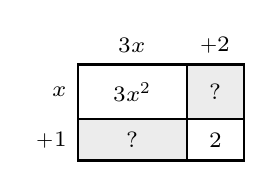
\begin{tikzpicture}[scale=0.66, every node/.style={font=\footnotesize, text=black}]
      \draw[black, line width=0.9pt, fill=white] (0,0.8) rectangle (2.1,1.85);
      \draw[black, line width=0.9pt, fill=gray!15] (2.1,0.8) rectangle (3.2,1.85);
      \draw[black, line width=0.9pt, fill=gray!15] (0,0) rectangle (2.1,0.8);
      \draw[black, line width=0.9pt, fill=white] (2.1,0) rectangle (3.2,0.8);
      \node at (1.05,1.325) {$3x^2$};
      \node at (2.65,1.325) {$?$};
      \node at (1.05,0.40) {$?$};
      \node at (2.65,0.40) {$2$};
      \node[above=0.5pt] at (1.05,1.85) {$3x$};
      \node[above=0.5pt] at (2.65,1.85) {$+2$};
      \node[left=0.5pt] at (0,1.325) {$x$};
      \node[left=0.5pt] at (0,0.40) {$+1$};
    \end{tikzpicture}
  \end{minipage}
\end{tcolorbox}

% -------------------- ផ្នែកទី២៖ E2 EXPLORE --------------------
\secbar{ផ្នែកទី២ ៖ រុករកវិធីគុណ និងវិធីចែកពហុធា \enbf{(E2 — Explore)}}{\en{11} នាទី (ពិភាក្សាដៃគូ)}

\textbf{ក. សកម្មភាពទី១ (រុករកវិធីគុណពហុធាតាមប្រអប់ផ្ទៃក្រឡា និងលក្ខណៈបំបែក ទំ.៥៩)៖}
\begin{enumerate}[label=\arabic*., leftmargin=0.55cm, itemsep=4pt, topsep=2pt]
  \item \textbf{ឧទាហរណ៍ទី១ (ឯកធា $\times$ ពហុធា)៖} ចតុកោណកែង \en{(I)} មានផ្ទៃក្រឡា $x\times 3x = \dotline{1.4cm}$ និងចតុកោណកែង \en{(II)} មានផ្ទៃក្រឡា $x\times 1 = \dotline{1.2cm}$ $\implies$ ផ្ទៃក្រឡាសរុប $x(3x + 1) = x(\dotline{1.1cm}) + x(\dotline{0.9cm}) = \dotline{2.5cm}$ ។
  \item \textbf{ឧទាហរណ៍ទី២ (ទ្វេធា $\times$ ទ្វេធា)៖} បំពេញប្រអប់សញ្ញា «$?$» ទាំងពីរខាងលើ រួចបូកបញ្ចូលគ្នា៖\\
  $(3x + 2)(x + 1) = 3x(x) + 3x(1) + 2(x) + 2(1) = 3x^2 + \dotline{1.3cm} + \dotline{1.3cm} + 2 = \dotline{3.5cm}$ ។
  \item \textbf{វិភាគកំហុស៖} ហេតុអ្វី $(3x + 2)(x + 1) \ne 3x^2 + 2$? ព្រោះបាត់ផ្ទៃក្រឡាប្រអប់ឆ្វែងទាំងពីរគឺ $\dotline{1.5cm}$ និង $\dotline{1.5cm}$ ។
\end{enumerate}

\vspace{4pt}
\textbf{ខ. សកម្មភាពទី២ (រុករកវិធីចែកពហុធានឹងឯកធា ទំ.៦០ និងប៉ូតង់ចែកពហុធា ទំ.៦១)៖}
\begin{enumerate}[label=\arabic*., leftmargin=0.55cm, itemsep=4.5pt, topsep=2pt]
  \item \textbf{ពហុធា $\div$ ឯកធា (ឧទាហរណ៍ទី២ ទំ.៦០)៖} ចែកគ្រប់តួនឹង $5x^2$៖
  $(15x^4 - 30x^6)\div 5x^2 = \dfrac{15x^4}{5x^2} - \dfrac{30x^6}{5x^2} = \dotline{3.2cm}$ ។
  \item \textbf{ប៉ូតង់ចែកដាច់ vs ចែកមានសំណល់ (ឧទាហរណ៍ទី៣ និងទី៤ ទំ.៦១)៖} បំពេញចន្លោះក្នុងប៉ូតង់ទាំងពីរ៖\par\vspace{3.5pt}
  \begin{minipage}[t]{9.2cm}
    \textbf{ករណីទី១ (ចែកដាច់)៖} $(x^2 - 7x + 10)\div(x - 2)$\\[2pt]
    $\begin{array}{r@{\;}l}
      x^2 - 7x + 10 & \multicolumn{1}{|l}{\;x - 2} \\ \cline{2-2}
      -\,(x^2 - 2x)\phantom{+10} & \;x - \dotline{0.9cm} \\ \cline{1-1}
      -\,5x + 10 & \\
      -\,(-\,5x + 10) & \\ \cline{1-1}
      \text{សំណល់ } = \dotline{0.9cm} & \implies \text{ផលចែក } = \dotline{1.8cm}
    \end{array}$
  \end{minipage}\hfill
  \begin{minipage}[t]{9.2cm}
    \textbf{ករណីទី២ (មានសំណល់)៖} $(x^2 - 2x + 4)\div(x - 1)$\\[2pt]
    $\begin{array}{r@{\;}l}
      x^2 - 2x + 4 & \multicolumn{1}{|l}{\;x - 1} \\ \cline{2-2}
      -\,(x^2 - x)\phantom{+4} & \;x - \dotline{0.9cm} \\ \cline{1-1}
      -\,x + 4 & \\
      -\,(-\,x + 1) & \\ \cline{1-1}
      \text{សំណល់ } = \dotline{0.9cm} & \implies \dfrac{x^2-2x+4}{x-1} = \dotline{2.4cm}
    \end{array}$
  \end{minipage}
\end{enumerate}

\vspace{2pt}
% -------------------- ផ្នែកទី៣៖ E3 EXPLAIN --------------------
\secbar{ផ្នែកទី៣ ៖ សង្ខេបវិធានគុណ-ចែកពហុធា និងធនាគារហេតុផល \enbf{(E3 — Explain)}}{\en{6} នាទី (កត់ត្រាខ្លឹមសារគោល)}

\begin{tcolorbox}[enhanced, sharp corners, colback=white, colframe=black, boxrule=0.85pt, top=4.5pt, bottom=4.5pt, left=6pt, right=6pt]
  \cnum{1} \textbf{គុណឯកធានឹងពហុធា (ទំ.៥៩)៖} គេគុណឯកធានឹង \dotline{2.3cm} នៃពហុធា រួចបង្រួមលទ្ធផល ។\\[3.5pt]
  \cnum{2} \textbf{គុណពហុធានឹងពហុធា (ទំ.៦០)៖} គេយកកត្តានីមួយៗនៃពហុធាទី១ គុណនឹង \dotline{2.5cm} នៃពហុធាទី២ រួចបង្រួមតួដូចគ្នា ។\\[3.5pt]
  \cnum{3} \textbf{ចែកពហុធានឹងឯកធា (ទំ.៦១)៖} គេចែក \dotline{2.3cm} នៃពហុធានឹងឯកធានោះ ។ \cnum{4} មុនចែកប៉ូតង់ ត្រូវរៀបដឺក្រេចុះ និងបំពេញខ្ទង់ $\mathbf{0x^k}$ ត្រង់ដឺក្រេដែលបាត់ ។\\[3.5pt]
  \cnum{5} \textbf{ទំនាក់ទំនងចែកមានសំណល់ (ទំ.៦១)៖} $\dfrac{\text{តំណាងចែក}}{\text{តួចែក}} = \dotline{2.2cm} + \dfrac{\dotline{2.2cm}}{\text{តួចែក}}$ (បើសំណល់ $=0$ ហៅថា \textbf{ចែកដាច់}) ។\\[4pt]
  \centering
  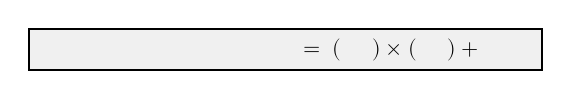
\begin{tikzpicture}
    \node[draw=black, line width=0.8pt, fill=panelgray, inner xsep=10pt, inner ysep=3.5pt, font=\footnotesize] {ផ្ទៀងផ្ទាត់ប្រមាណវិធីចែក៖ \quad $\text{តំណាងចែក} \;=\; (\text{តួចែក}) \times (\text{ផលចែក}) + \text{សំណល់}$};
  \end{tikzpicture}
\end{tcolorbox}

\newpage
% ============================================================================
% ទំព័រទី២៖ E4 (លំហាត់គំរូ ទំ.៦០, ៦២) + E5 (ប្រតិបត្តិ + Exit Check) + កិច្ចការផ្ទះ
% ============================================================================

% -------------------- ផ្នែកទី៤៖ E4 ELABORATE --------------------
\secbar{ផ្នែកទី៤ ៖ អនុវត្តលំហាត់គំរូតាមសៀវភៅគោល \enbf{(E4 — Elaborate)}}{\en{10} នាទី (បំពេញតាមគំរូ)}

\textbf{១. លំហាត់គំរូគុណពហុធា និងការសរសេរចំនួនគត់ជាពហុធានៃ $10$ (ទំ.៦០)៖}
\begin{itemize}[leftmargin=0.5cm, itemsep=3.5pt, topsep=2pt]
  \item \textbf{គំរូទី១៖} $3x^2(4x^3 + xy - 5y^2) = 3x^2(4x^3) + 3x^2(xy) - 3x^2(5y^2) = \dotline{5.6cm}$ ។
  \item \textbf{គំរូទី២ (គុណតាមជួរឈរ)៖} រៀប $1 + x^2 - 3x$ ជា $x^2 - 3x + 1$ រួចគុណនឹង $2x - 3$ ៖\\
  ជួរទី១៖ $(2x)(x^2 - 3x + 1) = \dotline{3.8cm}$ \;;\; ជួរទី២៖ $(-3)(x^2 - 3x + 1) = \dotline{3.8cm}$ \\
  បូកតម្រឹមដឺក្រេតាមជួរឈរ បានផលគុណស្មើ៖ $\dotline{6.2cm}$ ។
  \item \textbf{គំរូទី៣ (ទំ.៦០)៖} សរសេរ $7368$ ជាពហុធានៃ $10$៖ $7368 = 7\times 10^3 + \dotline{1.6cm} + \dotline{1.5cm} + \dotline{1.0cm}$ ។
\end{itemize}

\vspace{3pt}
\textbf{២. លំហាត់គំរូចែកពហុធាដែលបាត់ខ្ទង់ដឺក្រេកណ្ដាល (ទំ.៦២)៖} ចូរបំពេញប៉ូតង់ទាំងពីរដោយដាក់ខ្ទង់សូន្យជាមុន៖\par\vspace{3pt}
\begin{minipage}[t]{9.2cm}
  \textbf{គំរូទី១៖} $(8y^3 + 4y^2 + \mathbf{0y} - 7)\div(2y + 3)$\\[2pt]
  $\begin{array}{r@{\;}l}
    8y^3 + 4y^2 + \mathbf{0y} - 7 & \multicolumn{1}{|l}{\;2y + 3} \\ \cline{2-2}
    -\,(8y^3 + 12y^2)\phantom{+0y-7} & \;4y^2 - \dotline{1.0cm} + \dotline{0.9cm} \\ \cline{1-1}
    -\,8y^2 + \mathbf{0y} - 7 & \\
    -\,(-\,8y^2 - 12y)\phantom{-7} & \\ \cline{1-1}
    12y - 7 & \\
    -\,(12y + 18) & \\ \cline{1-1}
    \text{សំណល់ } = \dotline{1.1cm} &
  \end{array}$\\[2pt]
  ដូចនេះ លទ្ធផល $= \dotline{4.8cm}$ ។
\end{minipage}\hfill
\begin{minipage}[t]{9.2cm}
  \textbf{គំរូទី២៖} $(x^3 - 2)\div(x - 1) = (x^3 + \mathbf{0x^2} + \mathbf{0x} - 2)\div(x - 1)$\\[2pt]
  $\begin{array}{r@{\;}l}
    x^3 + \mathbf{0x^2} + \mathbf{0x} - 2 & \multicolumn{1}{|l}{\;x - 1} \\ \cline{2-2}
    -\,(x^3 - x^2)\phantom{+0x-2} & \;x^2 + \dotline{0.9cm} + \dotline{0.9cm} \\ \cline{1-1}
    x^2 + \mathbf{0x}\phantom{-2} & \\
    -\,(x^2 - x)\phantom{-2} & \\ \cline{1-1}
    x - 2 & \\
    -\,(x - 1) & \\ \cline{1-1}
    \text{សំណល់ } = \dotline{1.1cm} &
  \end{array}$\\[2pt]
  ដូចនេះ $\dfrac{x^3 - 2}{x - 1} = \dotline{4.8cm}$ ។
\end{minipage}

\vspace{3pt}
$\bullet$ \textbf{ឆ្លុះបញ្ចាំង (\en{Looking Back})៖} ផ្ទៀងផ្ទាត់ $(x - 1)(x^2 + x + 1) + (-1) = \dotline{3.8cm} - 1 = x^3 - 2$ (ពិត!) ។

% -------------------- ផ្នែកទី៥៖ E5 EVALUATE --------------------
\secbar{ផ្នែកទី៥ ៖ ហ្វឹកហាត់ «ប្រតិបត្តិ» និងតេស្តរហ័ស \enbf{(E5 — Evaluate)}}{\en{10} នាទី (ធ្វើដោយខ្លួនឯង រួចប្ដូរផ្ទៀង)}

\textbf{១. ប្រតិបត្តិគុណពហុធា (ទំ.៦០) និងប្រតិបត្តិចែកពហុធា (ទំ.៦២)៖}

\vspace{2pt}
{\renewcommand{\arraystretch}{1.38}
\begin{tabular}{|L{9.1cm}|L{9.1cm}|}
\hline
\cellcolor{headgray}\textbf{ប្រតិបត្តិគុណពហុធា (សៀវភៅគោល ទំ.៦០)} & \cellcolor{headgray}\textbf{ប្រតិបត្តិចែកពហុធា (សៀវភៅគោល ទំ.៦២)} \\
\hline
ក. $2x^2(2x^2 + 3x - 1) = \dotline{4.6cm}$ & ក. $(a^2b^3 + 2ab)\div(ab) = \dotline{4.4cm}$ \\
\hline
ខ. $ab^2(a^2 + 2ab + a) = \dotline{4.6cm}$ & ខ. $(5x^2y^4 + 2x^3y^5 - 12x^2y^2)\div(x^2y^2) = \dotline{3.1cm}$ \\
\hline
គ. $(a^2 + 2ab)(a - b) = \dotline{4.7cm}$ & គ. $(6x^2 + 5x - 4)\div(2x - 1) = \dotline{4.0cm}$ \\
\hline
ឃ. $(9a^2 - 25)(a^5 + ab) = \dotline{4.4cm}$ & ឃ. $(a^2 + 6a - 55)\div(a - 5) = \dotline{4.2cm}$ \\
\hline
ង. $\dfrac{1}{2}xy^2\left(\dfrac{2}{3}xy - 3\right) = \dotline{4.5cm}$ & ផ្ទៀងផ្ទាត់ ឃ៖ $(a-5)(\dotline{1.8cm}) = a^2 + 6a - 55$ \\
\hline
\end{tabular}}

\vspace{4pt}
\begin{tcolorbox}[enhanced, sharp corners, colback=panelgray, colframe=black, boxrule=0.85pt, top=3pt, bottom=3pt, left=6pt, right=6pt]
  \textbf{២. បិទបេសកកម្ម \en{E1} និងតេស្តរហ័ស (\en{Exit Check — 60} វិនាទី)៖}\\[2pt]
  $\bullet$ \textbf{ចម្លើយបេសកកម្ម \en{E1}៖} ផ្ទៃក្រឡារូបថតប្រាសាទគឺ $(3x+2)(x+1) = \dotline{3.5cm}$ (មានតួកណ្ដាល $+3x+2x = +5x$) ។\\[2pt]
  $\bullet$ \textbf{សំណួរតេស្តរហ័ស៖} តើផលគុណ $(2x - 3)(x + 4)$ ស្មើនឹងពហុធាមួយណា? (គូសរង្វង់ជម្រើសត្រឹមត្រូវ)\\[1.5pt]
  \hspace*{0.3cm}\enbf{A.}\; $2x^2 - 12$ \qquad\quad
  \enbf{B.}\; $2x^2 + 11x - 12$ \qquad\quad
  \enbf{C.}\; $2x^2 + 5x - 12$ \qquad\quad
  \enbf{D.}\; $2x^2 - 5x - 12$
\end{tcolorbox}

% -------------------- ផ្នែកទី៦៖ កិច្ចការផ្ទះ --------------------
\secbar{ផ្នែកទី៦ ៖ ប័ណ្ណកិច្ចការផ្ទះ \enbf{(Homework)} និងការអានជាមុន}{សៀវភៅសិក្សាគោល ទំ.៧២--៧៣}

\begin{tcolorbox}[enhanced, sharp corners, colback=white, colframe=black, boxrule=0.8pt, borderline={0.6pt}{2pt}{dashed}, top=3pt, bottom=3pt, left=6pt, right=6pt]
  \textbf{១. លំហាត់ទី៣ គ (ទាំង ២ ឃ្លា ទំ.៧២)៖} គណនាផលគុណ $(x^2 + 2y)(x + 1)$ និង $(x^2 - y)(y - 4)$ ។\\[1.5pt]
  \textbf{២. លំហាត់ទី៦ (ទំ.៧៣)៖} គណនា បង្រួម និងរៀបតាមលំដាប់ដឺក្រេចុះ៖ $a(x - b) - b(a - x) + x(a + b)$ ។\\[1.5pt]
  \textbf{៣. លំហាត់ទី៧ ក--ខ (ទំ.៧៣)៖} ក) $y(x+a-y) - a(x+y-a) - a(a^2+y^2)$ \;;\; ខ) $(t-1)(t-2) - (t+1)(t-3) - 2(t-2)(t+3)$ ។\\[1.5pt]
  $\bullet$ \textbf{អានជាមុន៖} ចំណុច \textbf{៣.១ សមភាពសំខាន់ៗ — ពន្លាតការេនៃទ្វេធា និងផលគុណទ្វេធាឆ្លាស់សញ្ញា} (សៀវភៅគោល ទំព័រ ៦៣--៦៦) ។
\end{tcolorbox}

\end{document}
